% The moseq-bxd project tree, drawn the way `tree` prints it, with a gloss per entry.
% Colours come from src/styles/palette.json via the generated ../_palette.tex (npm run tokens).
% Shared house style for the TikZ diagrams. render.sh defines \theme (light|dark) before \input.
\documentclass{article}
\usepackage{fontspec}
\usepackage{tikz}
\usepackage{fontawesome5}
\usetikzlibrary{positioning,calc,arrows.meta,fit,backgrounds}
\setmainfont{CrimsonPro}[Path=\fontdir, Extension=.ttf, UprightFont=*, ItalicFont=*-Italic, UprightFeatures={RawFeature={+wght=400}}, ItalicFeatures={RawFeature={+wght=400}}, BoldFont=*, BoldFeatures={RawFeature={+wght=600}}, Scale=1.08]
\setmonofont{JetBrainsMono}[Path=\fontdir, Extension=.ttf, Scale=0.86]
\newfontfamily\kickerfont{JetBrainsMono}[Path=\fontdir, Extension=.ttf, Scale=0.72, LetterSpace=12]
% GENERATED from src/styles/palette.json by scripts/tokens/build.mjs. Do not edit; run `npm run tokens`.
\def\darktheme{dark}
\ifx\theme\darktheme
  \definecolor{ink}{HTML}{EFEFE8}
  \definecolor{muted}{HTML}{A0A09A}
  \definecolor{paper}{HTML}{1B1B19}
  \definecolor{accent}{HTML}{5FE08F}
  \definecolor{accentfill}{HTML}{173322}
  \definecolor{oxide}{HTML}{FF6A4D}
\else
  \definecolor{ink}{HTML}{111111}
  \definecolor{muted}{HTML}{4A4A4A}
  \definecolor{paper}{HTML}{FFFFF8}
  \definecolor{accent}{HTML}{1F7A45}
  \definecolor{accentfill}{HTML}{E6F1EA}
  \definecolor{oxide}{HTML}{C8361C}
\fi

\tikzset{
  every picture/.style={line cap=round, line join=round, font=\normalsize, text=ink},
  card/.style={draw=ink!70!paper, line width=0.6pt, fill=paper, rounded corners=3pt, align=left,
               text width=#1, inner xsep=7pt, inner ysep=5.5pt, anchor=north west},
  card/.default=3.9cm,
  hot/.style={card=#1, draw=accent, line width=1.1pt, fill=accentfill},
  hot/.default=3.9cm,
  ghost/.style={card=#1, draw=muted!80!paper, dashed, fill=none, text=muted},
  ghost/.default=3.9cm,
  panel/.style={draw=muted!45!paper, line width=0.5pt, rounded corners=5pt, inner sep=9pt},
  hotpanel/.style={panel, draw=accent!75!paper, line width=0.9pt},
  line/.style={-{Stealth[length=5pt,width=4.2pt]}, line width=0.7pt, draw=ink!70!paper},
  hotline/.style={line, draw=accent, line width=1pt},
  ghostline/.style={line, draw=muted!80!paper, dashed},
  badline/.style={line, draw=oxide, line width=1pt},
  lbl/.style={font=\small\itshape, text=muted, inner sep=2.5pt},
  head/.style={font=\itshape, text=muted, anchor=south west, inner sep=0pt, align=left},
  warm/.style={card=#1, draw=accent!60!paper, fill=accentfill!50!paper},
  warm/.default=3.9cm,
}
\newcommand{\kicker}[1]{{\kickerfont\MakeUppercase{#1}}}
\newcommand{\ico}[1]{\makebox[1.25em][l]{#1}}
\newcommand{\cardtext}[2]{{\ttfamily #1}\\[1pt]{\small\itshape\color{muted}#2}}
% Crop the page to the picture: typeset it into a box and ship that box as the page.
\newcommand{\diagram}[1]{%
  \setbox0\hbox{#1}%
  \pagewidth=\dimexpr\wd0+8pt\relax \pageheight=\dimexpr\ht0+\dp0+8pt\relax
  \hoffset=-1in \voffset=-1in
  \shipout\vbox{\kern4pt\hbox{\kern4pt\box0}}}

\begin{document}
\diagram{\begin{tikzpicture}[x=1cm,y=-0.64cm]
  \def\ind{0.6}\def\gx{5.55}
  % the memory files sit on a tinted band
  \fill[accentfill, rounded corners=3pt] (0.3,0.52) rectangle (12.35,3.48);
  \node[font=\kickerfont\scriptsize, text=accent, anchor=south east, inner sep=0pt] at (12.3,0.4) {THE PROJECT'S MEMORY};
  % rails: (parent row, parent depth, last child row)
  \foreach \p/\d/\l in {0/0/13, 5/1/7, 8/1/10}
    \draw[ink!35!paper, line width=0.6pt] (\d*\ind+0.13,\p+0.38) -- (\d*\ind+0.13,\l);
  \foreach \r/\d in {1/1,2/1,3/1,4/1,5/1,6/2,7/2,8/1,9/2,10/2,11/1,12/1,13/1}
    \draw[ink!35!paper, line width=0.6pt] (\d*\ind-\ind+0.13,\r) -- (\d*\ind-0.1,\r);
  % rows
  \foreach \r/\d/\ic/\name/\gloss/\col in {
      0/0/folder-open/{moseq-bxd/}/{}/ink,
      1/1/file-alt/AGENTS.md/{the map: read first, every session}/accent,
      2/1/file-alt/CONCLUSIONS.md/{what we believe, and what we stopped believing}/accent,
      3/1/file-alt/WORKLOG.md/{what each session did, newest first}/accent,
      4/1/folder/{src/moseq\_bxd/}/{every reusable function lives here, tested}/ink,
      5/1/folder/{data/}/{}/ink,
      6/2/lock/{raw/}/{read-only (a hook refuses writes)}/muted,
      7/2/folder/{processed/}/{derived, safe to regenerate}/ink,
      8/1/folder/{experiments/}/{}/ink,
      9/2/file-alt/INDEX.md/{what has been tried, and how it came out}/ink,
      10/2/folder/{exp-NNNN\_slug/}/{one run, one folder, all of its outputs}/ink,
      11/1/folder/{notebooks/}/{looking around (never the source of a result)}/ink,
      12/1/folder/{deliverables/<slug>/}/{talks and papers, pointing back to their runs}/ink,
      13/1/folder/{docs/decisions/}/{why things are the way they are (ADRs)}/ink} {
    \node[text=\col, anchor=west, inner sep=0pt] (i) at (\d*\ind,\r) {\faIcon{\ic}};
    \node[text=\col, anchor=west, inner sep=0pt, font=\ttfamily] (n) at (\d*\ind+0.42,\r) {\name};
    \if\relax\detokenize\expandafter{\gloss}\relax\else
      \draw[muted!45!paper, line width=0.5pt, dash pattern=on 0.6pt off 2.4pt] ($(n.east)+(0.15,0)$) -- (\gx-0.15,\r);
      \node[lbl, anchor=west, inner sep=0pt] at (\gx,\r) {\gloss};
    \fi
  }
\end{tikzpicture}}
\end{document}
